\documentclass[11pt,a4paper,parskip=half]{scrreprt}

% ---------- Packages ----------
\usepackage[T1]{fontenc}
\usepackage[utf8]{inputenc}
\usepackage{lmodern}
\usepackage[a4paper,top=1.5cm,bottom=1.6cm,left=2cm,right=2cm,headsep=8pt]{geometry}
\usepackage[table]{xcolor}
\usepackage{booktabs}
\usepackage{array}
\usepackage{tabularx}
\usepackage{longtable}
\usepackage{amsmath}
\usepackage{amssymb}
\usepackage{enumitem}
\usepackage{fancyhdr}
\usepackage{tikz}
\usetikzlibrary{positioning,calc,shapes.geometric,backgrounds,patterns}
\usepackage[skins,breakable]{tcolorbox}
\usepackage{fontawesome5}
\usepackage{hyperref}
\usepackage{lastpage}

% ---------- Palette ----------
\definecolor{navy}{RGB}{15,23,42}
\definecolor{steel}{RGB}{47,98,137}
\definecolor{alert}{RGB}{178,42,55}
\definecolor{mist}{RGB}{240,244,248}
\definecolor{slate}{RGB}{100,116,139}
\definecolor{rlow}{RGB}{60,143,98}
\definecolor{rmed}{RGB}{214,166,44}
\definecolor{rhigh}{RGB}{224,120,42}
\definecolor{rcrit}{RGB}{178,42,55}

\hypersetup{
  colorlinks=true,
  linkcolor=steel,
  urlcolor=steel,
  citecolor=steel,
  pdftitle={Cybersecurity Architecture Specification},
  pdfauthor={Nexa Platform Security}
}

% ---------- Headings ----------
\setkomafont{disposition}{\normalfont\sffamily\bfseries\color{navy}}
\addtokomafont{section}{\Large}
\addtokomafont{subsection}{\large\color{steel}}
\addtokomafont{subsubsection}{\normalsize\color{slate}}
\setkomafont{descriptionlabel}{\sffamily\bfseries\color{steel}}
\renewcommand{\thesection}{\arabic{section}}
\RedeclareSectionCommand[beforeskip=1.4ex plus 0.4ex minus 0.4ex, afterskip=0.5ex plus 0.1ex]{section}
\RedeclareSectionCommand[beforeskip=1.0ex plus 0.3ex minus 0.3ex, afterskip=0.3ex]{subsection}

% ---------- Header / Footer ----------
\pagestyle{fancy}
\fancyhf{}
\renewcommand{\headrulewidth}{0.5pt}
\renewcommand{\footrulewidth}{0.4pt}
\fancyhead[L]{\small\sffamily\color{slate}Nexa Ledger Cloud Platform --- Security Architecture}
\fancyhead[R]{\small\sffamily\color{slate}NEXA-SEC-ARCH-2026-014}
\fancyfoot[L]{\small\sffamily\color{alert}CONFIDENTIAL --- INTERNAL DISTRIBUTION}
\fancyfoot[R]{\small\sffamily\color{slate}Page \thepage\ of \pageref{LastPage}}

% ---------- Helpers ----------
\newcommand{\risktag}[1]{%
  \ifcase#1
    \colorbox{rlow}{\textcolor{white}{\textbf{\small Low}}}%
  \or\colorbox{rlow}{\textcolor{white}{\textbf{\small Low}}}%
  \or\colorbox{rmed}{\textcolor{white}{\textbf{\small Medium}}}%
  \or\colorbox{rhigh}{\textcolor{white}{\textbf{\small High}}}%
  \or\colorbox{rcrit}{\textcolor{white}{\textbf{\small Critical}}}%
  \fi
}
\newcommand{\statusok}{\textcolor{rlow}{\textbf{\faLock\ Implemented}}}
\newcommand{\statuspart}{\textcolor{rmed}{\textbf{\faFile\ Partial}}}
\newcommand{\statusplan}{\textcolor{slate}{\textbf{\faPen\ Planned}}}

\newtcolorbox{infobox}[1][]{%
  colback=mist, colframe=steel, boxrule=0.6pt, arc=2pt,
  left=8pt, right=8pt, top=6pt, bottom=6pt, #1
}

\title{Cybersecurity Architecture Specification}
\author{Nexa Platform Security}
\date{}

\begin{document}

% ================= TITLE PAGE =================
\begin{titlepage}
\thispagestyle{empty}
\begin{tikzpicture}[remember picture,overlay]
  \fill[navy] (current page.north west) rectangle ([yshift=-3.6cm]current page.north east);
  \fill[steel] ([yshift=-3.6cm]current page.north west) rectangle ([yshift=-3.65cm]current page.north east);
  \node[anchor=north west,xshift=2cm,yshift=-1.1cm] at (current page.north west)
    {\color{white}\sffamily\Large Nexa Technologies \textbar\ Platform Security};
  \node[anchor=north west,xshift=2cm,yshift=-2.0cm] at (current page.north west)
    {\color{mist}\sffamily\small Enterprise Security Architecture Program};

  \begin{scope}[shift={($(current page.north east)+(-2.4cm,-1.85cm)$)}]
    \node[regular polygon,regular polygon sides=6,minimum size=1.5cm,draw=white,fill=alert,line width=1pt] (hex) {};
    \node[text=white] at (hex) {\sffamily\bfseries\faLock};
  \end{scope}
\end{tikzpicture}

\vspace{4.2cm}

\begin{center}
{\sffamily\bfseries\fontsize{28}{32}\selectfont\color{navy} Cybersecurity Architecture\\[2pt] Specification}\\[14pt]
{\sffamily\Large\color{steel} Nexa Ledger Cloud Platform --- Version 4.2}\\[6pt]
{\sffamily\large\color{slate} Trust Zones, Threat Model \& Compliance Control Mapping}
\end{center}

\vspace{1.6cm}

\begin{center}
\begin{tcolorbox}[colback=white,colframe=steel,boxrule=0.8pt,arc=3pt,width=0.82\textwidth,
  left=14pt,right=14pt,top=10pt,bottom=10pt]
\sffamily
\begin{tabularx}{\linewidth}{@{}l X@{}}
\textbf{\color{steel}Document ID:} & NEXA-SEC-ARCH-2026-014 \\
\textbf{\color{steel}Classification:} & Confidential --- Internal Distribution \\
\textbf{\color{steel}Version:} & 3.0 (Approved) \\
\textbf{\color{steel}Effective Date:} & 23 July 2026 \\
\textbf{\color{steel}Owner:} & Platform Security Architecture Team \\
\textbf{\color{steel}Review Cycle:} & Semi-annual, or upon material architecture change \\
\end{tabularx}
\end{tcolorbox}
\end{center}

\vfill

\begin{center}
\small\sffamily\color{slate}
Prepared by Marcus Chen, Lead Security Architect \textbar\ Reviewed by Priya Nair, Compliance \& Risk \textbar\ Approved by Elena Kowalski, CISO
\end{center}
\vspace{0.6cm}
\end{titlepage}

\pagestyle{fancy}

% ================= DOCUMENT CONTROL =================
\section*{Document Control}
\addcontentsline{toc}{section}{Document Control}

\subsection*{Revision History}
\par\noindent{
\footnotesize
\begin{tabularx}{\textwidth}{@{}l l l X@{}}
\toprule
\rowcolor{navy}
\textcolor{white}{\textbf{Version}} & \textcolor{white}{\textbf{Date}} & \textcolor{white}{\textbf{Author}} & \textcolor{white}{\textbf{Summary of Changes}} \\
\midrule
1.0 & 2025-11-04 & M.\ Chen & Initial trust-zone model and STRIDE baseline for Ledger Platform v3. \\
2.0 & 2026-03-17 & M.\ Chen & Added multi-region data residency zone; revised IAM section for workload identity federation. \\
2.1 & 2026-05-29 & P.\ Nair & Compliance mapping updated for SOC~2 Type II renewal scope. \\
3.0 & 2026-07-23 & M.\ Chen & Incorporated risk register heat map; approved for v4.2 release gate. \\
\bottomrule
\end{tabularx}
}
\par

\subsection*{Approval}
\par\noindent{
\footnotesize
\begin{tabularx}{\textwidth}{@{}X l l@{}}
\toprule
\rowcolor{steel}
\textcolor{white}{\textbf{Role}} & \textcolor{white}{\textbf{Name}} & \textcolor{white}{\textbf{Date}} \\
\midrule
Lead Security Architect (Author) & Marcus Chen & 2026-07-23 \\
Compliance \& Risk Manager (Reviewer) & Priya Nair & 2026-07-23 \\
Chief Information Security Officer (Approver) & Elena Kowalski & 2026-07-23 \\
\bottomrule
\end{tabularx}
}
\par

% ================= EXECUTIVE SUMMARY =================
\section{Executive Summary}

This specification defines the security architecture of the \textbf{Nexa Ledger Cloud Platform}, a
multi-tenant transaction-ledger and reconciliation service operated by Nexa Technologies. It
establishes the trust-zone segmentation model, the STRIDE-based threat model for the platform's
critical data paths, the identity and access control design, and the mapping of implemented
controls against SOC~2 Type II, ISO/IEC~27001:2022, and GDPR Article~32 requirements.

\begin{infobox}
\textbf{\color{navy}Scope.} This document covers the production environment (\texttt{ap-south-1}
primary, \texttt{eu-west-1} secondary) for the Ledger API, the Reconciliation Engine, and the
Customer Admin Console. It excludes internal corporate IT systems, which are governed by
NEXA-SEC-CORP-2024-002.
\end{infobox}

Since the v2.0 revision, the architecture has moved from a single flat VPC to a five-zone
segmentation model with workload-identity-based service-to-service authentication, closing three
of the four Critical findings from the 2026-Q1 penetration test. The remaining Critical finding
(unscoped admin session tokens) is tracked as \textbf{RISK-014} in Section~\ref{sec:risk} and is
gated for remediation prior to the v4.2 general-availability release.

% ================= ARCHITECTURE OVERVIEW =================
\section{Architecture Overview \& Trust Zones}
\label{sec:arch}

The platform is segmented into five trust zones with monotonically increasing sensitivity.
Traffic may only cross a zone boundary through an explicitly enumerated, authenticated gateway;
there is no direct routing between non-adjacent zones.

\par\noindent\begin{center}
\begin{tikzpicture}[
  zone/.style={rectangle, rounded corners=4pt, draw=steel, fill=mist, minimum width=12.6cm, minimum height=1.15cm, align=left, font=\sffamily\small},
  comp/.style={rectangle, rounded corners=2pt, draw=navy, fill=white, minimum height=0.85cm, font=\sffamily\scriptsize, inner sep=4pt, line width=0.6pt},
  lbl/.style={font=\sffamily\bfseries\scriptsize, color=steel, anchor=west},
  arr/.style={->, >=stealth, draw=slate, line width=0.8pt}
]

\node[zone] (z0) at (0,0) {};
\node[lbl] at ([xshift=6pt,yshift=7pt]z0.north west) {ZONE 0 --- PUBLIC INTERNET};
\node[comp] (internet) at ([xshift=2.4cm]z0.center) {\faGlobe\ Client Traffic};
\node[regular polygon, regular polygon sides=3, draw=alert, fill=alert!12, minimum size=0.55cm] (threat) at ([xshift=-4.6cm]z0.center) {};
\node[font=\sffamily\bfseries\scriptsize, color=alert] at (threat) {!};
\node[font=\sffamily\scriptsize, color=alert, anchor=west] at ([xshift=4pt]threat.east) {Threat Actor};

\node[zone] (z1) at (0,-2.05) {};
\node[lbl] at ([xshift=6pt,yshift=7pt]z1.north west) {ZONE 1 --- EDGE / PERIMETER};
\node[comp] (waf) at ([xshift=-2.6cm]z1.center) {\faLock\ WAF + CDN};
\node[comp] (ddos) at ([xshift=1.9cm]z1.center) {\faLock\ DDoS Scrubbing};

\node[zone] (z2) at (0,-4.1) {};
\node[lbl] at ([xshift=6pt,yshift=7pt]z2.north west) {ZONE 2 --- PUBLIC SUBNET (DMZ)};
\node[comp] (gw) at ([xshift=-2.6cm]z2.center) {\faServer\ API Gateway};
\node[comp] (lb) at ([xshift=1.9cm]z2.center) {\faServer\ Load Balancer};

\node[zone] (z3) at (0,-6.15) {};
\node[lbl] at ([xshift=6pt,yshift=7pt]z3.north west) {ZONE 3 --- APPLICATION SUBNET};
\node[comp] (auth) at ([xshift=-3.9cm]z3.center) {\faKey\ Auth Service};
\node[comp] (ledger) at ([xshift=-0.2cm]z3.center) {\faFile\ Ledger API};
\node[comp] (recon) at ([xshift=3.3cm]z3.center) {\faSearch\ Recon Engine};

\node[zone] (z4) at (0,-8.2) {};
\node[lbl] at ([xshift=6pt,yshift=7pt]z4.north west) {ZONE 4 --- DATA SUBNET (RESTRICTED)};
\node[comp] (db) at ([xshift=-2.6cm]z4.center) {\faDatabase\ Primary Ledger DB};
\node[comp] (kms) at ([xshift=1.9cm]z4.center) {\faLock\ KMS + Secrets};

\draw[arr] (internet) -- (waf);
\draw[arr] (waf) -- (gw);
\draw[arr] (ddos) -- (lb);
\draw[arr] (gw) -- (auth);
\draw[arr] (gw) -- (ledger);
\draw[arr] (lb) -- (recon);
\draw[arr] (ledger) -- (db);
\draw[arr] (recon) -- (db);
\draw[arr] (auth) -- (kms);

\draw[->, >=stealth, dashed, draw=alert, line width=0.9pt]
  (threat.south) .. controls +(0.1,-0.7) and +(-0.6,0.4) .. (waf.west);
\node[font=\sffamily\scriptsize\itshape, color=alert, anchor=east] at ([xshift=-4pt,yshift=2pt]waf.west) {blocked};

\begin{scope}[on background layer]
\fill[navy!5, draw=navy!25, rounded corners=6pt]
  ($(z0.north west)+(-0.3,0.3)$) rectangle ($(z4.south east)+(0.3,-0.3)$);
\end{scope}

\end{tikzpicture}

\small\sffamily\color{slate}\textbf{Figure 1.} Trust-zone segmentation for the Nexa Ledger Cloud Platform. Each zone boundary enforces mutual TLS and workload-identity authentication; the perimeter blocks unauthenticated lateral movement attempts before they reach the DMZ.
\end{center}
\par

\subsection{Zone Boundary Controls}
\par\noindent{
\small
\begin{tabularx}{\textwidth}{@{}l X l@{}}
\toprule
\rowcolor{navy}
\textcolor{white}{\textbf{Boundary}} & \textcolor{white}{\textbf{Enforced By}} & \textcolor{white}{\textbf{Auth Method}} \\
\midrule
Zone 0 $\rightarrow$ Zone 1 & Edge WAF rule sets, geo/IP reputation filtering, rate limiting & TLS 1.3 \\
Zone 1 $\rightarrow$ Zone 2 & Security group allow-list, signed CDN origin headers & mTLS \\
Zone 2 $\rightarrow$ Zone 3 & Service mesh sidecar policy, JWT audience validation & OAuth2 + mTLS \\
Zone 3 $\rightarrow$ Zone 4 & Database proxy IAM authentication, VPC endpoint policy & Workload identity \\
\bottomrule
\end{tabularx}
}
\par

% ================= THREAT MODEL =================
\section{Threat Model (STRIDE)}
\label{sec:stride}

Threats are enumerated per component along the primary transaction path (client
$\rightarrow$ API gateway $\rightarrow$ ledger service $\rightarrow$ primary database) using the
STRIDE taxonomy. Residual risk reflects likelihood and impact \emph{after} the listed mitigation.

\par\noindent{
\footnotesize
\begin{tabularx}{\textwidth}{@{}l X X c@{}}
\toprule
\rowcolor{navy}
\textcolor{white}{\textbf{Category}} & \textcolor{white}{\textbf{Threat}} & \textcolor{white}{\textbf{Mitigation}} & \textcolor{white}{\textbf{Residual}} \\
\midrule
Spoofing & Forged service-to-service calls impersonating the Ledger API & Short-lived workload identity certificates (SPIFFE/SVID), mutual TLS on every internal hop & \risktag{1} \\
Tampering & Reconciliation batch files altered in transit between Recon Engine and object storage & SHA-256 manifest signing, S3 object lock, append-only audit bucket & \risktag{1} \\
Repudiation & Admin disputes having approved a high-value ledger correction & Immutable action log with dual-control approval, signed with per-session key & \risktag{1} \\
Information Disclosure & Encryption keys recoverable from a compromised application host & Keys held only in KMS, never materialized on disk; envelope encryption at rest & \risktag{2} \\
Denial of Service & Volumetric flood against the public API Gateway & Edge scrubbing, adaptive rate limiting, autoscaled gateway tier & \risktag{2} \\
Elevation of Privilege & Unscoped admin session token reused across tenant boundaries & \textit{Partial --- tenant-scoped claims implemented; console-side enforcement pending (RISK-014)} & \risktag{4} \\
\bottomrule
\end{tabularx}
}
\par

% ================= DATA CLASSIFICATION =================
\section{Data Classification \& Flow}

\begin{description}[leftmargin=1.6cm, style=nextline]
\item[\textcolor{alert}{Restricted}] Ledger transaction records, bank account references, KMS key material. Encrypted at rest (AES-256-GCM, envelope encryption) and in transit (TLS 1.3). Access requires just-in-time elevation.
\item[\textcolor{rhigh}{Confidential}] Tenant configuration, reconciliation reports, audit logs. Encrypted at rest; access via role-scoped service accounts only.
\item[\textcolor{steel}{Internal}] Aggregated usage metrics, non-identifying telemetry. Standard access controls, no field-level encryption required.
\end{description}

Restricted data flows exclusively within Zones 3--4 and is never written to logs, caches, or the
Customer Admin Console's client-side state. Field-level tokenization is applied before any
Restricted value leaves the Ledger API's process boundary, including to the Reconciliation
Engine, which operates only on tokenized references.

% ================= IAM =================
\section{Identity \& Access Management}

\begin{minipage}[t]{0.48\textwidth}
\begin{tcolorbox}[colback=white,colframe=steel,arc=2pt,title={\sffamily\small Human Access},
  colbacktitle=steel, coltitle=white, boxrule=0.6pt]
\small
\begin{itemize}[leftmargin=1.4em]
\item SSO via SAML 2.0, enforced hardware-key MFA for all engineering and admin roles.
\item Just-in-time production access, 4-hour expiry, approved by second engineer.
\item Quarterly access recertification; auto-revoke on role change.
\end{itemize}
\end{tcolorbox}
\end{minipage}\hfill
\begin{minipage}[t]{0.48\textwidth}
\begin{tcolorbox}[colback=white,colframe=steel,arc=2pt,title={\sffamily\small Workload Access},
  colbacktitle=steel, coltitle=white, boxrule=0.6pt]
\small
\begin{itemize}[leftmargin=1.4em]
\item SPIFFE/SVID identities issued per service, rotated every 24 hours.
\item No long-lived static credentials in application configuration.
\item Database access brokered through IAM-authenticated proxy; no shared passwords.
\end{itemize}
\end{tcolorbox}
\end{minipage}
\par

% ================= COMPLIANCE MAPPING =================
\section{Compliance Control Mapping}
\label{sec:compliance}

\par\noindent{
\footnotesize
\begin{tabularx}{\textwidth}{@{}l l X l@{}}
\toprule
\rowcolor{navy}
\textcolor{white}{\textbf{Control ID}} & \textcolor{white}{\textbf{Framework(s)}} & \textcolor{white}{\textbf{Requirement}} & \textcolor{white}{\textbf{Status}} \\
\midrule
AC-02 & SOC~2 CC6.1, ISO~A.8.2 & Least-privilege role assignment, reviewed quarterly & \statusok \\
CR-05 & SOC~2 CC6.7, GDPR Art.~32 & Encryption of Restricted data at rest and in transit & \statusok \\
LG-03 & SOC~2 CC7.2, ISO~A.8.15 & Centralized, tamper-evident audit logging with 400-day retention & \statusok \\
IR-01 & SOC~2 CC7.3, ISO~A.5.24 & Documented incident response plan with defined severity tiers & \statusok \\
IAM-09 & SOC~2 CC6.3, ISO~A.8.5 & Tenant-scoped authorization enforced at every access point & \statuspart \\
DR-04 & GDPR Art.~17, ISO~A.5.33 & Verified data erasure across all replicas within 30 days & \statuspart \\
BC-02 & SOC~2 A1.2, ISO~A.5.29 & Cross-region failover tested at least twice annually & \statusplan \\
\bottomrule
\end{tabularx}
}
\par

\begin{infobox}
\textbf{\color{navy}Audit note.} IAM-09's partial status corresponds to RISK-014 (Section~\ref{sec:risk}).
The Customer Admin Console currently validates tenant scope server-side on read paths but not yet
on the bulk-export path; remediation is scheduled for the 2026-08 sprint ahead of the v4.2 GA gate.
\end{infobox}

% ================= RISK REGISTER =================
\section{Risk Register \& Heat Map}
\label{sec:risk}

\par\noindent\begin{center}
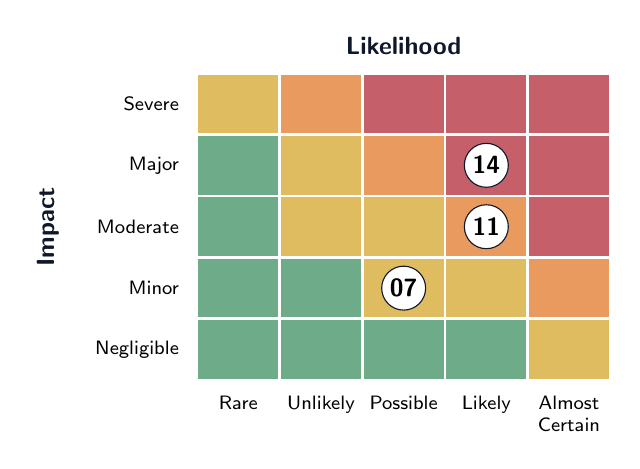
\begin{tikzpicture}[x=1.05cm,y=0.78cm]
\foreach \c/\i/\col in {
  1/1/rlow, 2/1/rlow, 3/1/rlow, 4/1/rlow, 5/1/rmed,
  1/2/rlow, 2/2/rlow, 3/2/rmed, 4/2/rmed, 5/2/rhigh,
  1/3/rlow, 2/3/rmed, 3/3/rmed, 4/3/rhigh, 5/3/rcrit,
  1/4/rlow, 2/4/rmed, 3/4/rhigh, 4/4/rcrit, 5/4/rcrit,
  1/5/rmed, 2/5/rhigh, 3/5/rcrit, 4/5/rcrit, 5/5/rcrit} {
  \fill[\col, fill opacity=0.75, draw=white, line width=1pt] (\c-0.5,\i-0.5) rectangle (\c+0.5,\i+0.5);
}
\node[font=\sffamily\bfseries\small, fill=white, draw=navy, circle, inner sep=1.5pt] at (4,4) {14};
\node[font=\sffamily\bfseries\small, fill=white, draw=navy, circle, inner sep=1.5pt] at (3,2) {07};
\node[font=\sffamily\bfseries\small, fill=white, draw=navy, circle, inner sep=1.5pt] at (4,3) {11};

\foreach \c/\txt in {1/Rare,2/Unlikely,3/Possible,4/Likely,5/Almost\\Certain}
  \node[font=\sffamily\scriptsize, anchor=north, align=center] at (\c,0.4) {\txt};
\foreach \i/\txt in {1/Negligible,2/Minor,3/Moderate,4/Major,5/Severe}
  \node[font=\sffamily\scriptsize, anchor=east] at (0.4,\i) {\txt};

\node[font=\sffamily\bfseries\small, color=navy, anchor=south] at (3,5.65) {Likelihood};
\node[font=\sffamily\bfseries\small, color=navy, anchor=south, rotate=90] at (-1.05,3) {Impact};
\end{tikzpicture}

\small\sffamily\color{slate}\textbf{Figure 2.} Risk heat map. Circled markers correspond to entries in the risk register below.
\end{center}
\par

\par\noindent{
\footnotesize
\begin{tabularx}{\textwidth}{@{}l X l l@{}}
\toprule
\rowcolor{steel}
\textcolor{white}{\textbf{ID}} & \textcolor{white}{\textbf{Description}} & \textcolor{white}{\textbf{Owner}} & \textcolor{white}{\textbf{Rating}} \\
\midrule
RISK-007 & Reconciliation batch retry storms during upstream bank outage & Recon Platform Team & \risktag{2} \\
RISK-011 & Credential-stuffing attempts against tenant admin login & Auth Team & \risktag{3} \\
RISK-014 & Bulk-export path lacks server-side tenant-scope enforcement & Marcus Chen & \risktag{4} \\
\bottomrule
\end{tabularx}
}
\par

% ================= MONITORING =================
\section{Monitoring, Logging \& Incident Response}

All Zone 2--4 components emit structured logs to a centralized, append-only log store with
400-day retention; Restricted-data fields are redacted at the logging shim before transmission.
Detection rules cover credential-stuffing patterns, anomalous cross-tenant query volume, and
KMS key-usage spikes, each mapped to a PagerDuty severity tier. Confirmed Severity-1 incidents
trigger the documented response plan: containment within 30 minutes, tenant notification within
72 hours where GDPR Article~33 applies, and a blameless post-incident review published to the
engineering org within five business days.

% ================= SIGN-OFF =================
\section*{Approval \& Sign-off}
\addcontentsline{toc}{section}{Approval \& Sign-off}

\noindent This architecture specification is approved for the v4.2 release gate, contingent on
remediation of RISK-014 prior to general availability.

\vspace{0.8cm}
\noindent
\begin{minipage}[t]{0.48\textwidth}
\rule{\linewidth}{0.4pt}\\[2pt]
Marcus Chen, Lead Security Architect
\end{minipage}\hfill
\begin{minipage}[t]{0.48\textwidth}
\rule{\linewidth}{0.4pt}\\[2pt]
Elena Kowalski, Chief Information Security Officer
\end{minipage}
\par

\end{document}
